\documentclass[compress,dvipsnames]{beamer}\usepackage[]{graphicx}\usepackage[]{xcolor}
% maxwidth is the original width if it is less than linewidth
% otherwise use linewidth (to make sure the graphics do not exceed the margin)
\makeatletter
\def\maxwidth{ %
  \ifdim\Gin@nat@width>\linewidth
    \linewidth
  \else
    \Gin@nat@width
  \fi
}
\makeatother

\definecolor{fgcolor}{rgb}{0.345, 0.345, 0.345}
\newcommand{\hlnum}[1]{\textcolor[rgb]{0.686,0.059,0.569}{#1}}%
\newcommand{\hlstr}[1]{\textcolor[rgb]{0.192,0.494,0.8}{#1}}%
\newcommand{\hlcom}[1]{\textcolor[rgb]{0.678,0.584,0.686}{\textit{#1}}}%
\newcommand{\hlopt}[1]{\textcolor[rgb]{0,0,0}{#1}}%
\newcommand{\hlstd}[1]{\textcolor[rgb]{0.345,0.345,0.345}{#1}}%
\newcommand{\hlkwa}[1]{\textcolor[rgb]{0.161,0.373,0.58}{\textbf{#1}}}%
\newcommand{\hlkwb}[1]{\textcolor[rgb]{0.69,0.353,0.396}{#1}}%
\newcommand{\hlkwc}[1]{\textcolor[rgb]{0.333,0.667,0.333}{#1}}%
\newcommand{\hlkwd}[1]{\textcolor[rgb]{0.737,0.353,0.396}{\textbf{#1}}}%
\let\hlipl\hlkwb

\usepackage{framed}
\makeatletter
\newenvironment{kframe}{%
 \def\at@end@of@kframe{}%
 \ifinner\ifhmode%
  \def\at@end@of@kframe{\end{minipage}}%
  \begin{minipage}{\columnwidth}%
 \fi\fi%
 \def\FrameCommand##1{\hskip\@totalleftmargin \hskip-\fboxsep
 \colorbox{shadecolor}{##1}\hskip-\fboxsep
     % There is no \\@totalrightmargin, so:
     \hskip-\linewidth \hskip-\@totalleftmargin \hskip\columnwidth}%
 \MakeFramed {\advance\hsize-\width
   \@totalleftmargin\z@ \linewidth\hsize
   \@setminipage}}%
 {\par\unskip\endMakeFramed%
 \at@end@of@kframe}
\makeatother

\definecolor{shadecolor}{rgb}{.97, .97, .97}
\definecolor{messagecolor}{rgb}{0, 0, 0}
\definecolor{warningcolor}{rgb}{1, 0, 1}
\definecolor{errorcolor}{rgb}{1, 0, 0}
\newenvironment{knitrout}{}{} % an empty environment to be redefined in TeX

\usepackage{alltt}

% Load ttbeamer template depending on operating system
\usepackage{ifplatform}
\ifwindows
	\usepackage{M:/pc/Dokumenter/ttbeamer}
\fi
\iflinux
	\usepackage{/home/tony/uio/pc/Dokumenter/ttbeamer}
\fi
\ifmacosx
	\usepackage{/Users/tctan/uio/pc/Dokumenter/ttbeamer}
\fi

\title{Lab 2 - Validity}
\author[]{Tony Tan \& Jarl Kristensen \\\vspace{6pt} {\em{University of Oslo}} }
\date{Monday, 14 November 2022}
\IfFileExists{upquote.sty}{\usepackage{upquote}}{}
\begin{document}



\begin{frame}[fragile]
\titlepage
\end{frame}


\begin{frame}[fragile]
	\frametitle{Today}
		\begin{itemize}
			\item Classical validity analysis using \ttemph{multitrait-multimethod matrix} (MTMM)
			\item Examine \ttemph{convergent validity} and \ttemph{discriminant validity}
			\item MTMM's relevance depends on intended \ttemph{interpretations} and \ttemph{uses} of the test scores
		\end{itemize}
\end{frame}


\begin{frame}[fragile]
	\frametitle{MTMM: Background}
		\begin{itemize}
			\item First proposed by \textcite{campbell:1959}
			\item Origin in personality (or \textcolor{red}{trait})	psychology
			\item Involving examining \ttemph{convergent} and \ttemph{discriminant} validity
				\begin{itemize}
					\item Convergent validity: Scores of \emph{same trait} measured by \emph{different methods} should correlate sufficiently strongly
					\item Discriminant validity: \emph{Different traits} measured by the \emph{same methods} should not correlate more strongly than above
				\end{itemize}
			\item A method for providing evidence pertaining to the \ttemph{relations to other variables} category of the \textit{Standards} \parencite{standards:2014}
		\end{itemize}
\end{frame}

\begin{frame}[fragile]
	\frametitle{MTMM: Structure}
	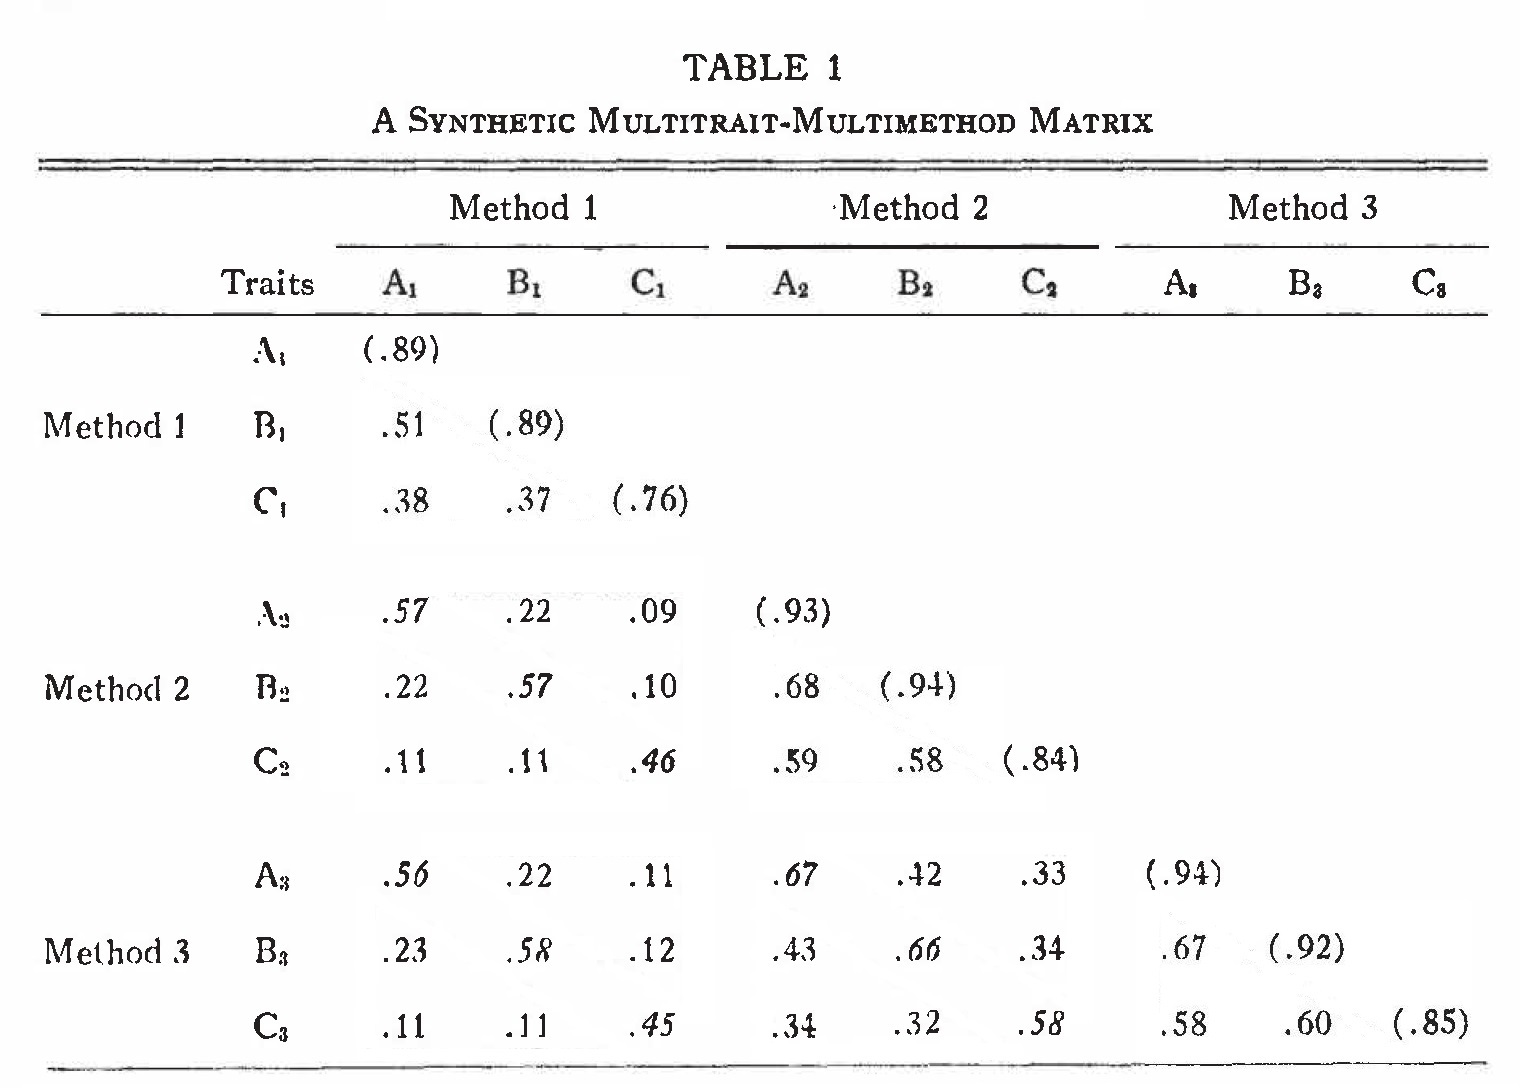
\includegraphics[width=\textwidth]{MTMM.jpg}
\end{frame}


\begin{frame}[fragile]
	\frametitle{Convergent validation}
		\begin{itemize}
			\item \textcolor{LimeGreen}{Reliability coefficient}: The proportion of variance shared between \ttemph{true scores} and \ttemph{observed scores} produced when a trait is measured by way of one specific method.
			\item \textcolor{CarnationPink}{Validity coefficient}: Correlation between trait scores produced by means of \ttemph{one method} should correlate strongly with those produced using \ttemph{another method}.
		\end{itemize}
\end{frame}


\begin{frame}[fragile]
	\frametitle{Discriminant validation}
		\begin{itemize}
			\item \textcolor{SkyBlue}{Between-trait, within-method correlation}: Correlation between scores on different traits measured using the \ttemph{same method}
			\item \textcolor{Dandelion}{Between-trait, between-method correlations}: Correlation between scores on different traits measured sing \ttemph{different methods}
		\end{itemize}
\end{frame}


\begin{frame}[fragile]
	\frametitle{MTMM validation criteria}
		\begin{enumerate}
			\item \textcolor{CarnationPink}{Validity diagonal} values should be
				\begin{itemize}
					\item statistically significant, and
					\item sufficiently large.
				\end{itemize}
			\item \textcolor{CarnationPink}{Validity diagonal} values should be higher than \textcolor{Dandelion}{heterotrait-heteromethod triangles}.
			\item Within each \textcolor{red}{heteromethod block}, correlation of the \colorbox{ForestGreen}{same trait} should be higher than correlations between \colorbox{Yellow}{different traits}.
			\item The same pattern of trait interrelationship should be evident in all heterotrait triangles of both the \textcolor{SkyBlue}{monomethod} and \textcolor{Dandelion}{heteromethod} blocks
		\end{enumerate}

		Criterion 1 = Convergent validity

		Criteria 2--4 = Discriminant validity
\end{frame}


\begin{frame}[fragile]
	\frametitle{Task 1: MTMM analysis}
		\begin{itemize}
			\item Download \pk{pomlab02.RData} from Canvas and load it into \cR
			\item These are MTMM matrices presented in \poscite{campbell:1959} original paper
			\item Conduct convergent and discriminant validation organised in the MTMM matrix
				\begin{itemize}
					\item Examine convergence and discriminant validities for the first method
					\item Examine convergence and discriminant validities for the second method
					\item Examine convergence and discriminant validities across methods
				\end{itemize}
		\end{itemize}
\end{frame}


\begin{frame}[fragile]
	\frametitle{``Disattenuating'' correlations}
		Correlations between scores are often impacted by imperfect reliability (``attenuation''). To get a ``true correlation'' between traits, we may correct for attenuation (``disattenuation'').

		\begin{itemize}
			\item Let $\rho_{xy}$ denote true correlation between traits $x$ and $y$ (``true''/perfect reliability).
			\item Let $r_{xy}$ denote the observed correlation between traits $x$ and $y$.
			\item Let $r_{xx}$ and $r_{yy}$ denote the reliabilities with which $x$ and $y$ are measured respectively.
		\end{itemize}

		An estimate of the ``true'' correlation between traits $x$ and $y$ can be obtained by:
		\[ \hat{\rho}_{xy} = \frac{r_{xy}}{\sqrt{r_{xx} r_{yy}}}. \]
\end{frame}


\begin{frame}[fragile]
	\frametitle{Task 2: MTMM disattenuation}
		\begin{itemize}
			\item Select one trait from the \pk{mtmm} matrix
				\begin{itemize}
					\item Examine convergence and discriminant validities for the first method
					\item Examine convergence and discriminant validities for the second method
					\item Examine convergence and discriminant validities across methods
				\end{itemize}
		\end{itemize}
\end{frame}









\begin{frame}[fragile]
	\frametitle{References}
	\printbibliography
\end{frame}

\end{document}
